\documentclass{article}

\usepackage[T2A]{fontenc} % Кодировка шрифта
\usepackage[utf8]{inputenc} % Кодировка ввода
\usepackage[english,russian]{babel} % Языковые настройки
\usepackage{graphicx} % Для вставки изображений
\usepackage{amsmath} % Для использования математических формул
\usepackage{amssymb}
\usepackage{cancel}
\usepackage{tikz}
\usepackage{amsfonts} % Для использования математических символов и шрифтов
\usepackage{titlesec} % Для настройки заголовков разделов
\usepackage{titling} % Для настройки титульной страницы
\usepackage{geometry} % Для настройки размеров страницы
\usepackage{pgfplots}
\usepackage{mdframed} % Для создания рамок

\pgfplotsset{compat=1.9}

% Настройка заголовков разделов
\titleformat{\section}
{\normalfont\Large\bfseries}{\arabic{section}}{1em}{}
\titleformat{\subsection}
{\normalfont\large\bfseries}{}{1em}{}

% Настройка титульной страницы
\setlength{\droptitle}{-3em} % Отступ заголовка
\title{\vspace{-1cm}Контрольная работа №6, задание 1}
\author{Вершинин Данил Алексеевич}
\date{\today}

% Настройка размеров страницы
\geometry{a4paper, margin=2cm}

\begin{document}
	\maketitle
	\subsection{Условие}
		Дано нелинейное уравнение: $16x^5+24x^3-2x^2-11 = 0$. Отделить корни. Предложить сходящийся метод простой итерации для уточнения корня. Оценить, хотя бы грубо, скорость сходимости. Построить итерационный процесс по методу Ньютона.
	\subsection{Решение}
	%TODO сделать отделение корней (можно по предрассчету)%
	\begin{figure}[h]
		\centering
		\begin{tikzpicture}
			
			
			\draw[thick, ->] (-2*2,0) -- (2*2,0) node[below] {$\Re(z)$};
			\draw[thick, ->] (0,-2*2) -- (0,2*2) node[left] {$\Im(z)$};
			
			\filldraw (1*2,0) circle (1pt) node[above]{1};
			\filldraw (0,1*2) circle (1pt) node[left]{i};
			\draw (0,0) -- (0.09408799815214919*2,2 *1.256160052262912);
			\draw (0,0) -- (0.09408799815214919*2,2 *-1.256160052262912);
			\draw (0,0) -- (-0.45393578883367447*2,2 *0.6292479954643618);
			\draw (0,0) -- (-0.45393578883367447*2,2 *-0.6292479954643618);
			\draw (0,0) -- (-0.45393578883367447*2,2 *0.6292479954643618);
			\filldraw (0.09408799815214919*2,2 *1.256160052262912) circle (2pt) node[right]{(0.094+1.256i)};
			\filldraw (0.09408799815214919*2,2 *-1.256160052262912) circle (2pt) node[right]{(0.094-1.256i)};
			\filldraw (-0.45393578883367447*2,2 *0.6292479954643618) circle (2pt) node[left]{(-0.454+0.629i)};
			\filldraw (-0.45393578883367447*2,2 *-0.6292479954643618) circle (2pt) node[left]{(-0.454-0.629i)};
			\filldraw (0.7196955813634115*2,2 *0) circle (2pt) node[below]{0.720};
			
			% Направления биссектрис
			% Первая биссектриса
			\coordinate (B1) at ({2*(1 + 0.09408799815214919)}, {2*(0 + 1.256160052262912)});
			% Вторая биссектриса
			\coordinate (B2) at ({2*(1 + 0.09408799815214919)}, {2*(0 - 1.256160052262912)});
			% Третья биссектриса
			\coordinate (B3) at ({1.5*(- 0.45393578883367447)}, {2.5*(0 + 0.9892479954643618)});
			% Четвертая биссектриса
			\coordinate (B4) at ({1.5*(- 0.45393578883367447)}, {2.5*(0 - 0.9892479954643618)});
			\coordinate (B5) at (-4, 0);
			
			% Биссектрисы
			\draw[dashed, red] (0,0) -- (B1);
			\draw[dashed, red] (0,0) -- (B2);
			\draw[dashed, red] (0,0) -- (B3);
			\draw[dashed, red] (0,0) -- (B4);
			\draw[dashed, red, ultra thick] (0,0) -- (B5);
			
			
			
			
			
			
		\end{tikzpicture}
		\caption{Корни уравнения. Область поиска разделена.}
		
	\end{figure}
	Предложим метод итерации:
	$$16x^5+24x^3-2x^2-11 = 0$$
	$$16x^5+24x^3=2x^2+11 \  \Rightarrow \ x^3 (16x^2+24) = 2x^2+11 \  \Rightarrow \ x^3 = \frac{2x^2+11}{16x^2+24}$$
	$$\phi(x_n) = x_{n+1} = \sqrt[3]{\frac{2x_n^2+11}{16x_n^2+24}}$$
	Найдём производную полученной функции:
	\[\left(\sqrt[3]{\frac{2x_n^2+11}{16x_n^2+24}}\right)' = \frac{1}{3}\cdot \left(\frac{2x_n^2+11}{16x_n^2+24}\right)^{-\frac{2}{3}}\times \frac{4x(16x^2+24) - 32x(2x^2+11)}{(16x^2+24)^2}\]
	\begin{figure}[h]
		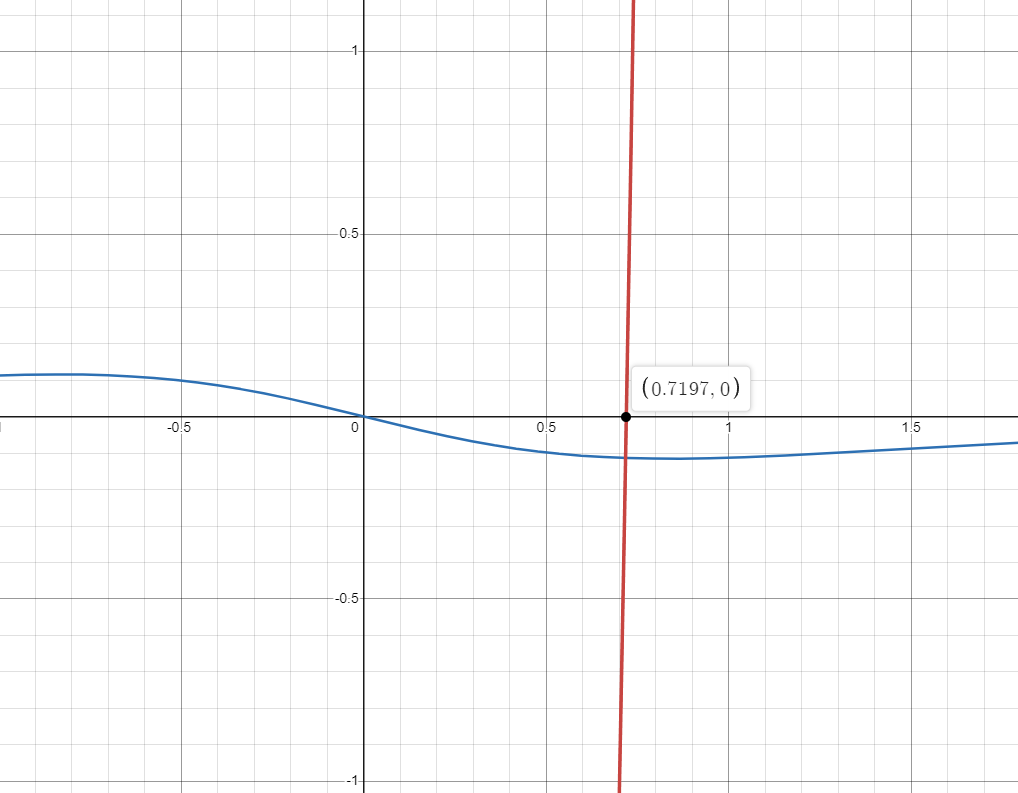
\includegraphics[width=150mm,scale=0.6]{iterations1.png}
		\caption{функция из уравнения (красный). Производная предложенного метода итераций (синий)}
	\end{figure}
	\newline
	На Рис. 2 показано, что функция, задающая уравнение, имеет только один вещественный корень. Заметим, что производная предложенной функции итерации по модулю всегда меньше единицы. Что позволяет нам сделать вывод о сходимости предложенной функции в окрестности вещественного корня (см Рис 3.). 
	\begin{figure}[h]
		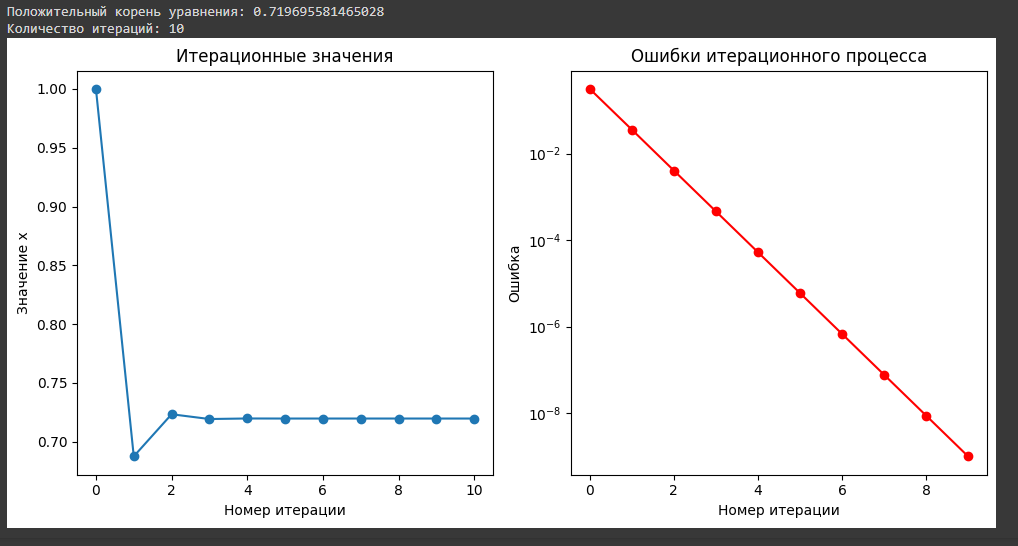
\includegraphics[width=160mm,scale=0.7]{iterations1_2.png}
		\caption{Вывод программы (см приложение [1]). За счёт того, что производная окрестности корня отрицательная, мы "перескакиваем" через корень. Метод имеет линейную скорость}
	\end{figure}
	\newpage
	\subsection{Метод Ньютона}
	Функцию дважды дифференцируема. Можно применить метод Ньютона.\newline
	
	Для применения метода Ньютона построим итерационную формулу:
	\begin{mdframed}
	\[x_{n+1} = x_n - \frac{f(x_n)}{f'(x_n)}\]\end{mdframed}
	Построим нашу функцию:
	\[x_{n+1} = x_n - \frac{16x_n^5+24x_n^3-2x_n^2-11}{80x_n^{4}+72x_n^{2}-4x_n}\]
	Результаты этого метода (использовалась программа [2]):
	\begin{verbatim}

		0.09408799815214919+1.256160052262912i
		0.09408799815214919-1.256160052262912i
		-0.45393578883367447+0.6292479954643618i
		-0.45393578883367447-0.6292479954643618i
		0.7196955813634115
	\end{verbatim}
	\newpage
	\subsection{Приложение}
	[1] Код на python для расчетов метода простой итерации 
	\begin{verbatim}
		import numpy as np
		import matplotlib.pyplot as plt
		import sympy as sp
		xx = sp.symbols('x')
		f = sp.root((2*xx**2 + 11) / (16*xx**2 + 24), 3)
		
		
		# Функция итерационного процесса
		def phi(x_i):
		return f.subs(xx, x_i)
		
		# Параметры итерационного процесса
		x0 = 1.0  # Начальное приближение
		tolerance = 1e-9  # Допуск
		max_iterations = 100  # Максимальное количество итераций
		
		# Массивы для хранения значений
		x_values = [x0]
		errors = []
		
		# Итерационный процесс
		for n in range(max_iterations):
		x_next = phi(x_values[-1])
		x_values.append(x_next)
		error = abs(x_next - x_values[-2])
		errors.append(error)
		if error < tolerance:
		break
		
		# Печать результатов
		print(f"Положительный корень уравнения: {x_values[-1]}")
		print(f"Количество итераций: {len(x_values) - 1}")
		
		# Визуализация сходимости
		plt.figure(figsize=(10, 5))
		
		plt.subplot(1, 2, 1)
		plt.plot(x_values, marker='o')
		plt.title("Итерационные значения")
		plt.xlabel("Номер итерации")
		plt.ylabel("Значение x")
		
		plt.subplot(1, 2, 2)
		plt.plot(errors, marker='o', color='r')
		plt.yscale('log')
		plt.title("Ошибки итерационного процесса")
		plt.xlabel("Номер итерации")
		plt.ylabel("Ошибка")
		
		plt.tight_layout()
		plt.show()
		
		
	\end{verbatim}

	[2] Код на python для расчетов методом Ньютона
	\begin{verbatim}
		f = lambda z: 16*z**5 + 24*z**3 -2*z**2-11
		df = lambda z: 80*z**4 + 72*z**2 - 4*z
		
		def newton_method_complex(f, df, z0, tol=1e-6, max_iter=1000):
		z = z0
		for i in range(max_iter):
		z_next = z - f(z) / df(z)
		if abs(z_next - z) < tol:
		print(i)
		return z_next
		z = z_next
		raise ValueError("Не удалось достичь сходимости")
		
		# Начальные приближения (включая комплексные)
		initial_guesses_complex = [0 + 1j, 0 - 1j, -1 + 1j, -1 - 1j, 1 + 0j]
		
		# Нахождение корней комплексным методом Ньютона
		complex_roots = []
		for guess in initial_guesses_complex:
		try:
		root = newton_method_complex(f, df, guess)
		if not any(np.isclose(root, r, atol=1e-6) for r in complex_roots):
		complex_roots.append(root)
		except ValueError:
		pass
		
		print("Найденные корни методом Ньютона:")
		for root in complex_roots:
		print(root)
	\end{verbatim}
	
	
	
\end{document}
